\chapter{Kurzanalyse}
\label{chapter-analyse}

Für die Entwicklung eines Dating-Protokolls ist es zwingend notwendig, eine Analyse der geistig verwirrten Hobby-Coaches durchzuführen.
Dabei soll verstanden werden, was der arme Timmy in den nächsten Stunden seines Dating-Coaching durchmachen muss und welche groben Fehler seitens der Coaches begangen werden.
Wer an dieser Stelle einen Methodik-Teil erwartet haben, wird diese nicht bekommen.
Schließlich muss sich auf das subjektive Niveau der YouTuber begeben werden, um diese auch analysieren zu können.
Im zweiten Abschnitt wird eine Marktanalyse mit random Fakts getätigt.

\section{Die Youtube-Szene}
\label{chapter-analyse-yt}

Die Plattform Youtube bietet Menschen die Möglichkeit Videos anzusehen, zu bewerten, zu kommentieren und hochzuladen. 
Diese hat eine sehr große Reichweite, sodass folglich auch für das Dating Videos produziert, hochgeladen und konsumiert werden.
Es kann jedermann zu jeder Zeit ein Video zu einem beliebigen Thema veröffentlichen.
Hierbei geht es nicht um Wissen, sondern um die Anzahl der Klicks, da oftmals die Einnahmen im Vordergrund stehen.
Damit einher geht, dass der Suchalgorithmus primär die Videos vorschlägt, die viele Aufrufe haben.
Verwendet man nun den Suchbegriff \glqq Frauen überzeugen\grqq~fällt eine besondere Technik dabei auf – Clickbaiting.
Die Abbildung \ref{fig:analyse-clickbait} zeigt den ersten Suchvorschlag des Algorithmus, wobei das Clickbaiting deutlich wird.
In dem Falle werden vorrangig gutaussehende Frauen mit großen Überschriften und teils mit weitem Ausschnitt oder sexueller Pose dargestellt. 

\begin{figure}[h]
    \centering
    
\includegraphics[scale=0.4]{Sources/clickbait.png}
    \caption{Klassisches Thumbnail mit Clickbaiting-Komponenten \cite{royalflushseduction}}
    \label{fig:analyse-clickbait}
\end{figure}

Als Nächstes werden die konkreten Inhalte analysiert.
Das beispielhafte Video von \glqq Flirt-Forschung\grqq, natürlich ein männlicher YouTuber, erläutert die Einteilung der Frauen in drei Gruppen \cite{royalflushseduction}.
Diese hängt davon ab, wie viele Alternativen die Frau neben dem Mann hat.
Je weniger Alternativen in Form von Männern eine Frau hat, desto einfacher soll das Dating sein.
Im Falle von vielen Alternativen muss der Typ überzeugend sein, um eine Chance zu haben.
Das heißt für den armen Timmy, dass er keine Probleme beim Dating hat.
Der arme Timmy hat nämlich einen großen Penis und ein Sixpack.

TODO


\section{Marktanalyse Singlebörsen}

Inzwischen gibt es in Deutschland über 2500 Singlebörsen auf denen Singles, darunter unser kleiner Timmy, ihre Partnersuche bestreiten \cite{kundler}.
Zu diesen gehören Plattformen wie Tinder, Bumble, Fremdgehen69 und Paarship.
Der geschätzte Umsatz im Bereich der Singlebörsen wird für dieses Jahr (2022) auf knapp 97 Millionen Euro geschätzt \cite{statista}.
Der Umsatz soll laut Prognose weiter steigen und im Jahr 2027 auf 102,5 Millionen Euro steigen.
Anhand der in Abbildung \ref{fig:analyse-alter} dargestellten Altersstruktur der Nutzenden lässt sich ableiten, dass dem armen Timmy die Singlebörsen verwehrt bleiben.

\begin{figure}[h]
    \centering
    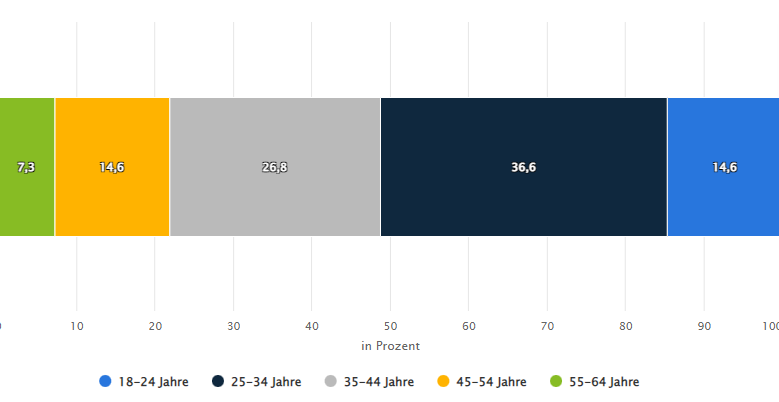
\includegraphics[scale=0.52]{Sources/alter.png}
    \caption{Nutzende nach Alter in Deutschland aus Oktober 2021 \cite{statista}.}
    \label{fig:analyse-alter}
\end{figure}

Dabei scheinen die jungen Erwachsenen (18-24 Jahre) am wenigstens verzweifelt zu sein.
Das ist weniger verwunderlich, da dieses Alter viele soziale Ausflüge, beispielsweise Dorfpartys und Shishabars, zulässt.
Den Hauptteil bildet die Altersgruppe von 25 bis 34 Jahre.
Dies lässt sich ebenso leicht erklären, schließlich hat der Zahn der Zeit auch an der Jugendliebe gekratzt.
Ein leichter Rückgang ist im Alter von 35 bis 44 zu erkennen.
Dabei handelt es sich um Menschen, die sich mit 20 Jahren verheiratet haben.
Diese merken nun auch, dass der Partner nicht mehr so frisch ist, aber mussten aufgrund der Ehe\footnote{Steuerliche Vorteile} und dem gesellschaftlichen Druck noch eine Weile durchhalten.
Ist dieser Punkt allerdings, warum auch immer, überstanden, fängt das gefährliche Alter von 45 bis 54 Jahre an.
Schätzungen zufolge soll diese Altersgruppe sehr anfällig für Seitensprünge sein \cite{seitensprung}.
Ab dem Alter von 65 Jahren gibt es offensichtlich keine Nutzer mehr.
Dies beruht auf mindestens einem der folgenden Gründe:
\begin{itemize}
    \item Das Altersheim bietet genug Auswahl
    \item Beide bereits gestorben
    \item Defizite in der Handhabung mit Technik
    \item Der demente Partner vergisst sowieso innerhalb von einer halben Stunde, wenn Uschi da war.
\end{itemize} 
Nach Statista betrugt im Oktober 2021 der weibliche Nutzeranteil der Singlebörsen in Deutschland nur 30,5 \% \cite{statista}.
Verwunderlich ist dies wohl kaum, da nur 22 \% Pferdemänner\footnote{Nicht zu verwechseln mit Deckhengsten vom Fickstutenmarkt} den Reitsport ausmachen \cite{bliemel}.

Für den armen Timmy ist demnach nichts dabei.
Das ist auch gut so, schließlich wird er erst im November 14 Jahre alt.
Die Altersgruppen scheinen alle ihre Probleme zu haben, wobei die jungen Erwachsenen am besten abschneiden.
Generell verwenden alle volljährige Altersgruppen Singlebörsen\footnote{bis zu einem gewissen Alter}. 
Daher ist die wichtigste Anforderung an das zu entwickelnde Protokoll, dass es zeitlos und allgemein ist.
Zudem ist in Abschnitt \ref{chapter-analyse-yt} deutlich geworden, dass Dating-Coaches auf YouTube sexistischer als Mario Barth sind und veraltete Klischees bedienen.